\documentclass[]{tufte-handout}

% ams
\usepackage{amssymb,amsmath}

\usepackage{ifxetex,ifluatex}
\usepackage{fixltx2e} % provides \textsubscript
\ifnum 0\ifxetex 1\fi\ifluatex 1\fi=0 % if pdftex
  \usepackage[T1]{fontenc}
  \usepackage[utf8]{inputenc}
\else % if luatex or xelatex
  \makeatletter
  \@ifpackageloaded{fontspec}{}{\usepackage{fontspec}}
  \makeatother
  \defaultfontfeatures{Ligatures=TeX,Scale=MatchLowercase}
  \makeatletter
  \@ifpackageloaded{soul}{
     \renewcommand\allcapsspacing[1]{{\addfontfeature{LetterSpace=15}#1}}
     \renewcommand\smallcapsspacing[1]{{\addfontfeature{LetterSpace=10}#1}}
   }{}
  \makeatother

\fi

% graphix
\usepackage{graphicx}
\setkeys{Gin}{width=\linewidth,totalheight=\textheight,keepaspectratio}

% booktabs
\usepackage{booktabs}

% url
\usepackage{url}

% hyperref
\usepackage{hyperref}

% units.
\usepackage{units}


\setcounter{secnumdepth}{2}

% citations


% pandoc syntax highlighting

% table with pandoc
\usepackage{longtable,booktabs,array}
\usepackage{calc} % for calculating minipage widths
% Correct order of tables after \paragraph or \subparagraph
\usepackage{etoolbox}
\makeatletter
\patchcmd\longtable{\par}{\if@noskipsec\mbox{}\fi\par}{}{}
\makeatother
% Allow footnotes in longtable head/foot
\IfFileExists{footnotehyper.sty}{\usepackage{footnotehyper}}{\usepackage{footnote}}
\makesavenoteenv{longtable}

% multiplecol
\usepackage{multicol}

% strikeout
\usepackage[normalem]{ulem}

% morefloats
\usepackage{morefloats}


% tightlist macro required by pandoc >= 1.14
\providecommand{\tightlist}{%
  \setlength{\itemsep}{0pt}\setlength{\parskip}{0pt}}

% title / author / date
\title{20 minutes of glucose metabolism}
\author{markwallace.org/teaching/glucose}
\date{}

%\geometry{showframe}% for debugging purposes -- displays the margins

%Switch fonts
%\usepackage[sfdefault,condensed]{roboto}
%\usepackage[sfdefault,light,condensed]{roboto}
%\usepackage{libertineRoman}
%\usepackage{libertineRoman}
%\usepackage{mweights}
\usepackage[sfdefault,light]{merriweather}

%Fix paragraph indent
\usepackage[parfill]{parskip}

%Fix Page colour
\pagecolor{white}

%Fix Section Heading fonts sizes and spacing.
\usepackage{titlesec}
%\newfontfamily\headingfont[]{Gill Sans} % Specify different font for section headings
\titleformat{\section}{\sffamily\LARGE\bfseries}{\thesection}{1em}{}[]
\titleformat{\subsection}{\sffamily\Large\bfseries}{\thesubsection}{1em}{}[]
\titlespacing{\section}{0pt}{\parskip}{0pt}
\titlespacing{\subsection}{0pt}{\parskip}{0pt}
\titlespacing{\subsubsection}{0pt}{\parskip}{0pt}

%Fix Title fonts sizes and spacing.
\usepackage{titling}
\setlength{\droptitle}{-80pt}
\pretitle{ \begin{fullwidth}\begin{flushleft}\Huge\sffamily\bfseries}
\posttitle{\par\end{flushleft}\vskip 0.5em \end{fullwidth}}
\preauthor{\begin{flushleft}\LARGE\sffamily}
\postauthor{\par\end{flushleft}\vskip 0.5em}
\predate{\begin{flushleft}\Large\sffamily}
\postdate{\par\end{flushleft}\vskip 0.5em}

%Attempt to fix ugly font for equation numberign
\makeatletter
\def\tagform@#1{\maketag@@@{\sffamily[\ignorespaces#1\unskip\@@italiccorr]}}
\renewcommand{\eqref}[1]{\textup{{\normalfont(\ref{#1}}\normalfont)}}
\makeatother

\begin{document}

\maketitle


\setlength{\parindent}{0pt}



Glucose is your primary metabolic fuel. Your brain depends on glucose as its main source of energy. Humans need a way of regulating the amount of available glucose, and like every biological machine, the ways your body goes about solving this problem results in a complex and multiplex system of regulation. Central to that regulation is the liver. One of its primary jobs is to serve as the main buffer for blood glucose concentration regulation.

\subsection{Pathway Overview}\label{pathway-overview}

\begin{figure}

{\centering \includegraphics{img/glucose_pathways_summary} 

}

\caption[Summary overview over primary glucose pathways]{Summary overview over primary glucose pathways.}\label{fig:unnamed-chunk-1}
\end{figure}

\subsection{Definitions}\label{definitions}

\textbf{Glycogenolysis}: The enzymatic breakdown of glycogen into glucose monomers or glucose-1-phosphate. It serves as a rapid source of glucose during times of energy need, such as exercise or fasting.

\textbf{Glycogenesis}: Glycogenesis is the process of synthesizing glycogen from glucose molecules. It allows the storage of excess glucose for future energy needs, maintaining blood glucose levels within a narrow range.

\textbf{Gluconeogenesis}: Gluconeogenesis is the formation of glucose from non-carbohydrate precursors, such as amino acids, lactate, or glycerol. It helps maintain blood glucose levels during fasting periods or low-carbohydrate intake by providing glucose for energy to tissues that depend on it, such as the brain.

\textbf{Glycolysis}: Glycolysis is the metabolic pathway that breaks down glucose into pyruvate, generating ATP and NADH as energy carriers. It is a central process in cellular respiration, providing energy for various cellular activities and serving as a precursor for other metabolic pathways.

\subsection{A closer look at Glycogen}\label{a-closer-look-at-glycogen}

Glycogen is the polysaccharide that serves as a storage form of glucose. It consists of glucose units linked together in a highly branched structure. Upon demand, glycogen can be rapidly broken down into glucose through glycogenolysis, providing a quick source of energy. Its structure allows for efficient storage and release of glucose

\begin{marginfigure}

{\centering 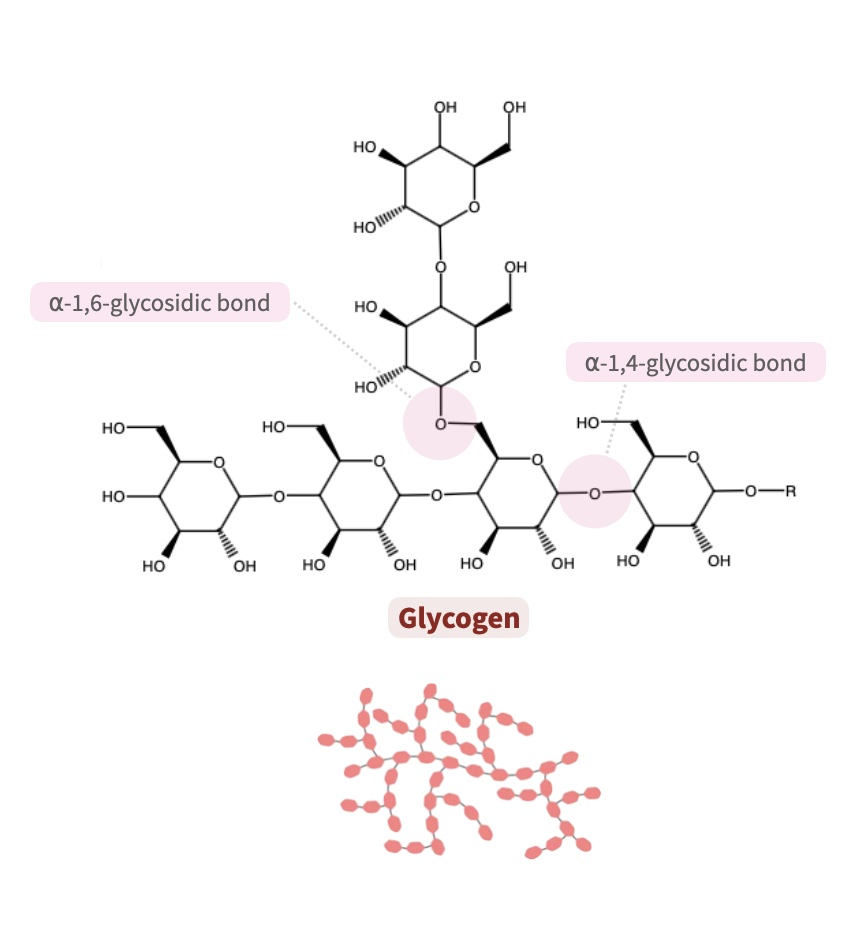
\includegraphics{img/glycogen} 

}

\caption[The structure of Glycogen]{The structure of Glycogen.}\label{fig:unnamed-chunk-2}
\end{marginfigure}

\subsection{Glycogenesis}\label{glycogenesis}

Glucose is converted into glycogen through a process called glycogenesis, which primarily occurs in the liver (and muscle cells). During glycogenesis, glucose molecules are phosphorylated to glucose-6-phosphate by the enzyme hexokinase. Then, glucose-6-phosphate is converted to glucose-1-phosphate by phosphoglucomutase. Subsequently, glucose-1-phosphate is activated by the enzyme UDP-glucose pyrophosphorylase to form UDP-glucose, which serves as the substrate for glycogen synthesis. Glycogen synthase then catalyzes the elongation of glycogen chains by adding UDP-glucose units, forming \(\alpha\)-1,4-glycosidic linkages.

\begin{figure}

{\centering 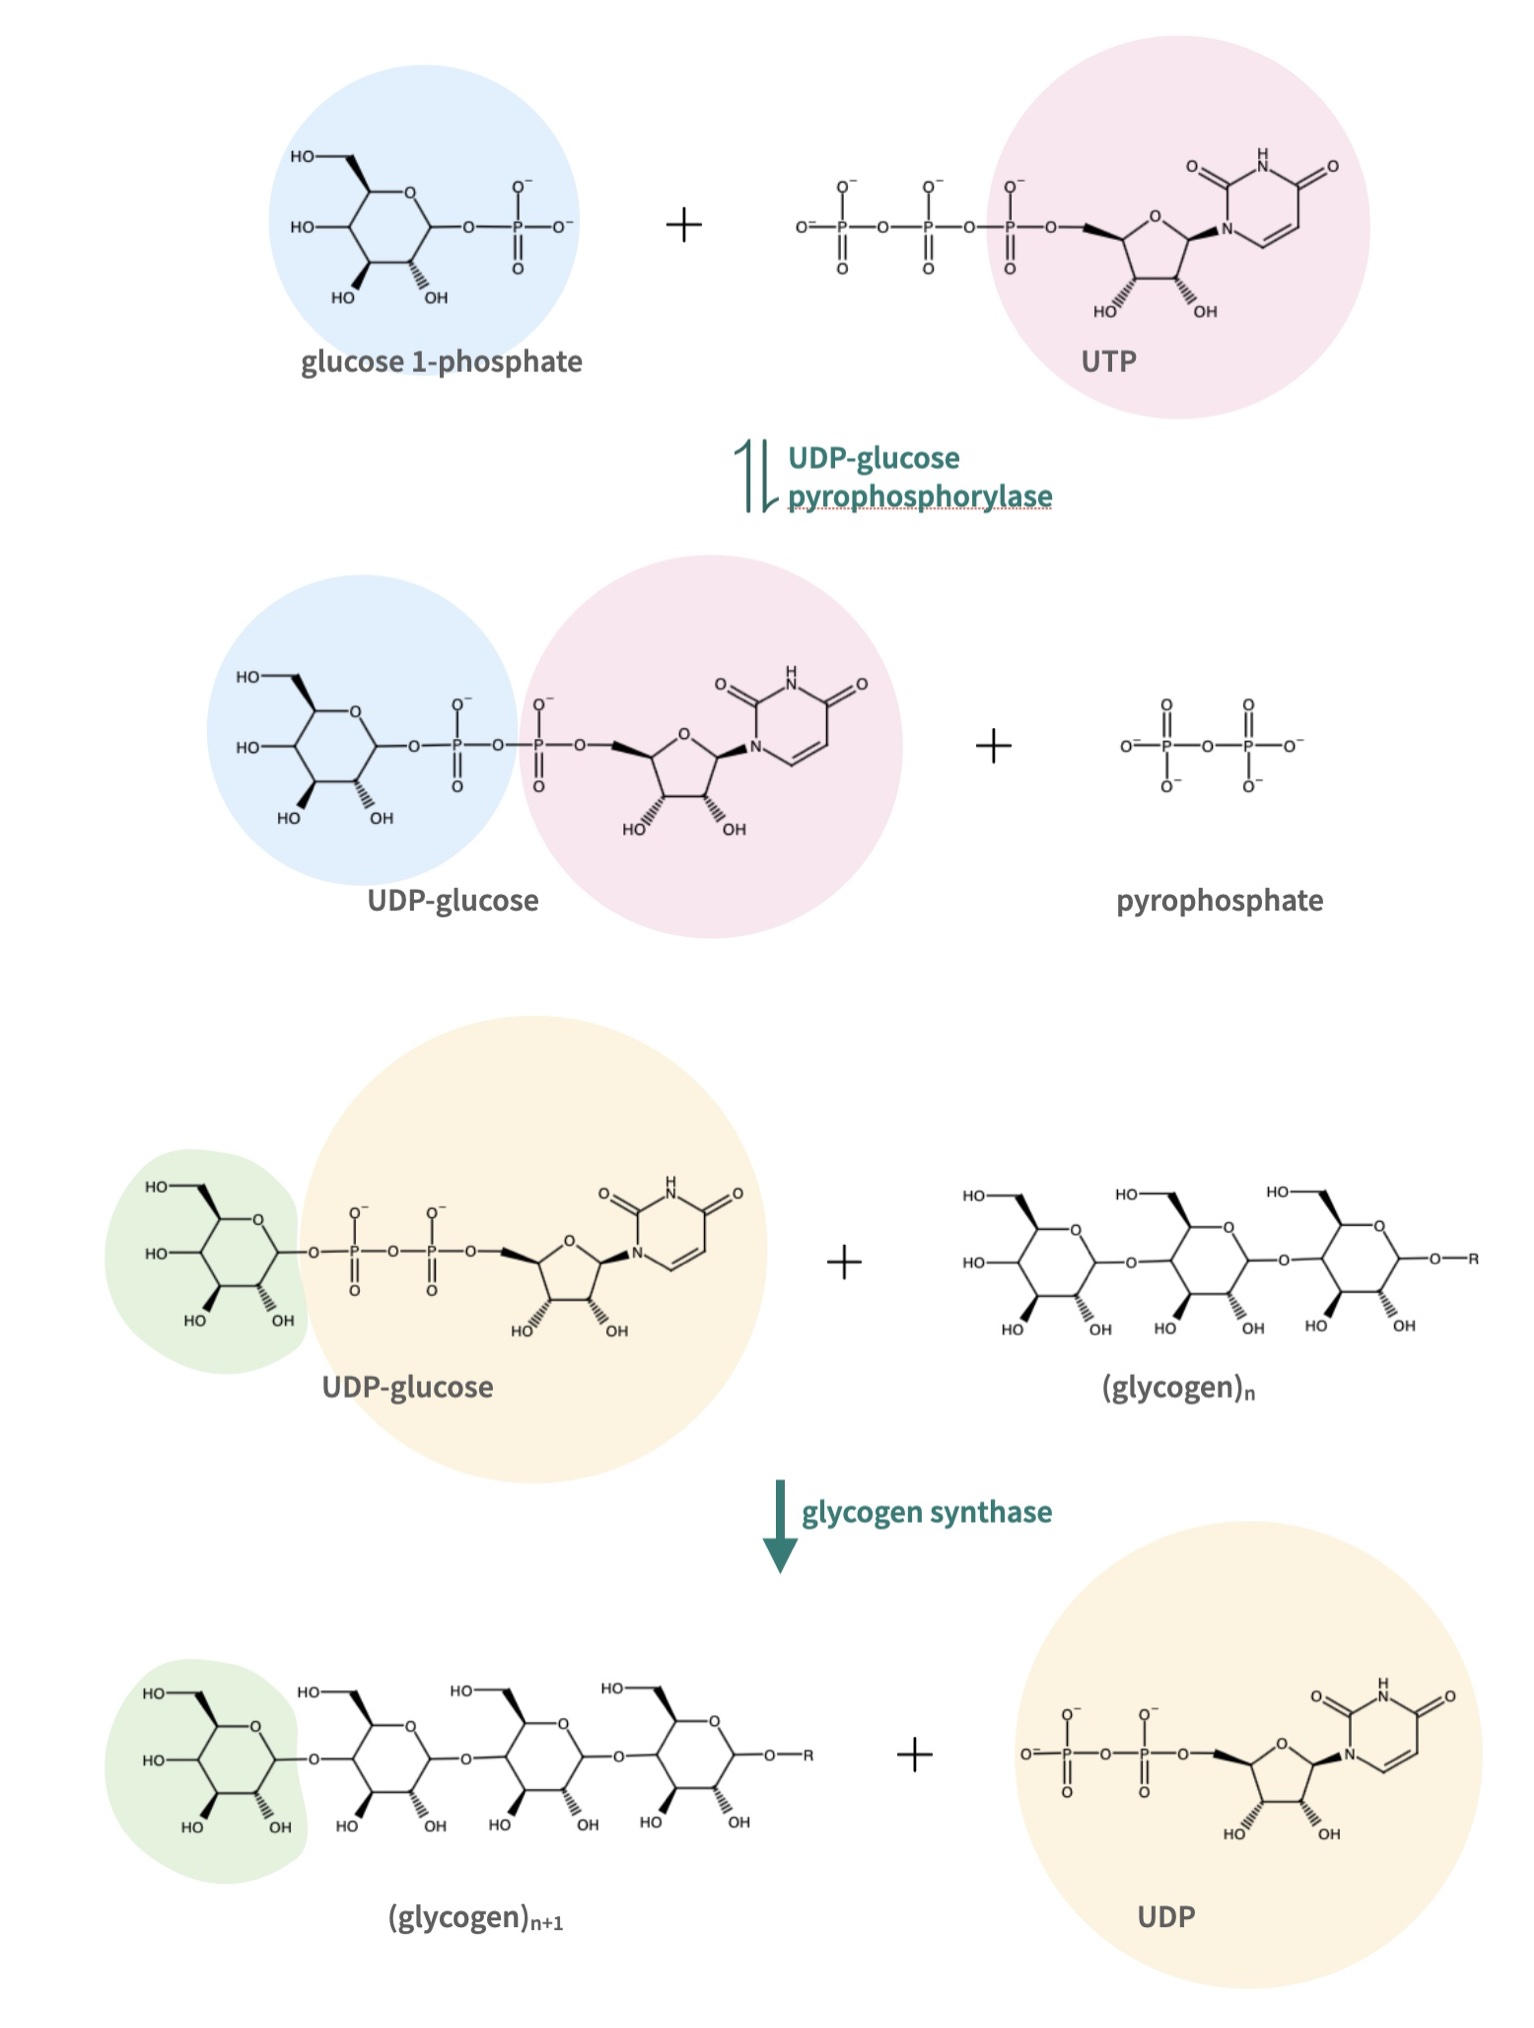
\includegraphics{img/glyogenesis} 

}

\caption[Glycogenesis is the process of synthesizing glycogen from glucose molecules]{Glycogenesis is the process of synthesizing glycogen from glucose molecules.}\label{fig:unnamed-chunk-3}
\end{figure}

\subsection{Glycogenolysis}\label{glycogenolysis}

The breakdown of glycogen back into glucose is facilitated by the process of glycogenolysis. Glycogenolysis involves the sequential removal of glucose units from the glycogen molecule. Glycogen phosphorylase cleaves glucose units from the outer branches of glycogen, producing glucose-1-phosphate. The enzyme phosphoglucomutase then converts glucose-1-phosphate to glucose-6-phosphate. Glucose-6-phosphatase catalyzes the dephosphorylation of glucose-6-phosphate in the liver to release free glucose into the bloodstream. This glucose can then be released into the bloodstream to maintain blood glucose levels.

\begin{figure}

{\centering 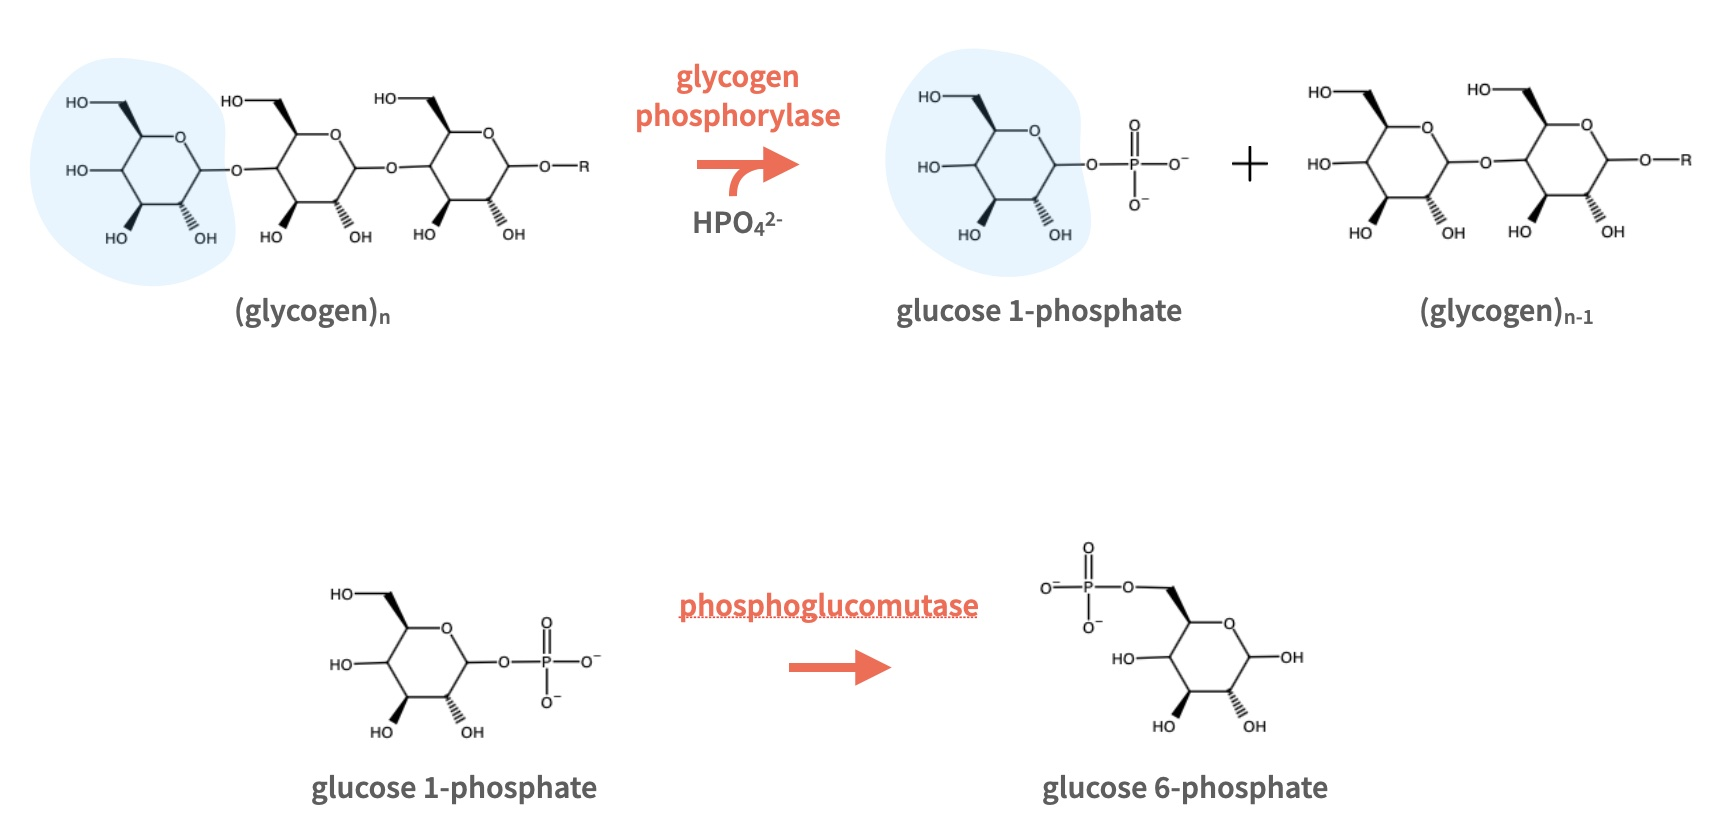
\includegraphics{img/glyogenolysis} 

}

\caption[Glycogenolysis is the enzymatic breakdown of glycogen into glucose monomers or glucose-1-phosphate]{Glycogenolysis is the enzymatic breakdown of glycogen into glucose monomers or glucose-1-phosphate. }\label{fig:unnamed-chunk-4}
\end{figure}

\subsection{Regulation}\label{regulation}

These processes must be carefully regulated in order to maintain glucose levels in the blood. This regulation can be homeostatic, and e.g., driven directly by glucose concentration, or via the action of hormones such as Insulin and Glucagon.

\subsection{Insulin and Glucagon}\label{insulin-and-glucagon}

Insulin and glucagon are hormones that play crucial roles in regulating blood glucose levels. Insulin is released by the pancreas in response to high blood glucose levels, promoting the uptake of glucose by cells, thus lowering blood sugar levels. It also stimulates the conversion of glucose into glycogen for storage in the liver and muscles. In contrast, glucagon is released when blood glucose levels are low, promoting the breakdown of glycogen into glucose through glycogenolysis, thus raising blood sugar levels. Together, insulin and glucagon maintain glucose homeostasis in the body, ensuring cells have a steady supply of energy while preventing excessively high or low blood sugar levels.

\begin{figure}

{\centering 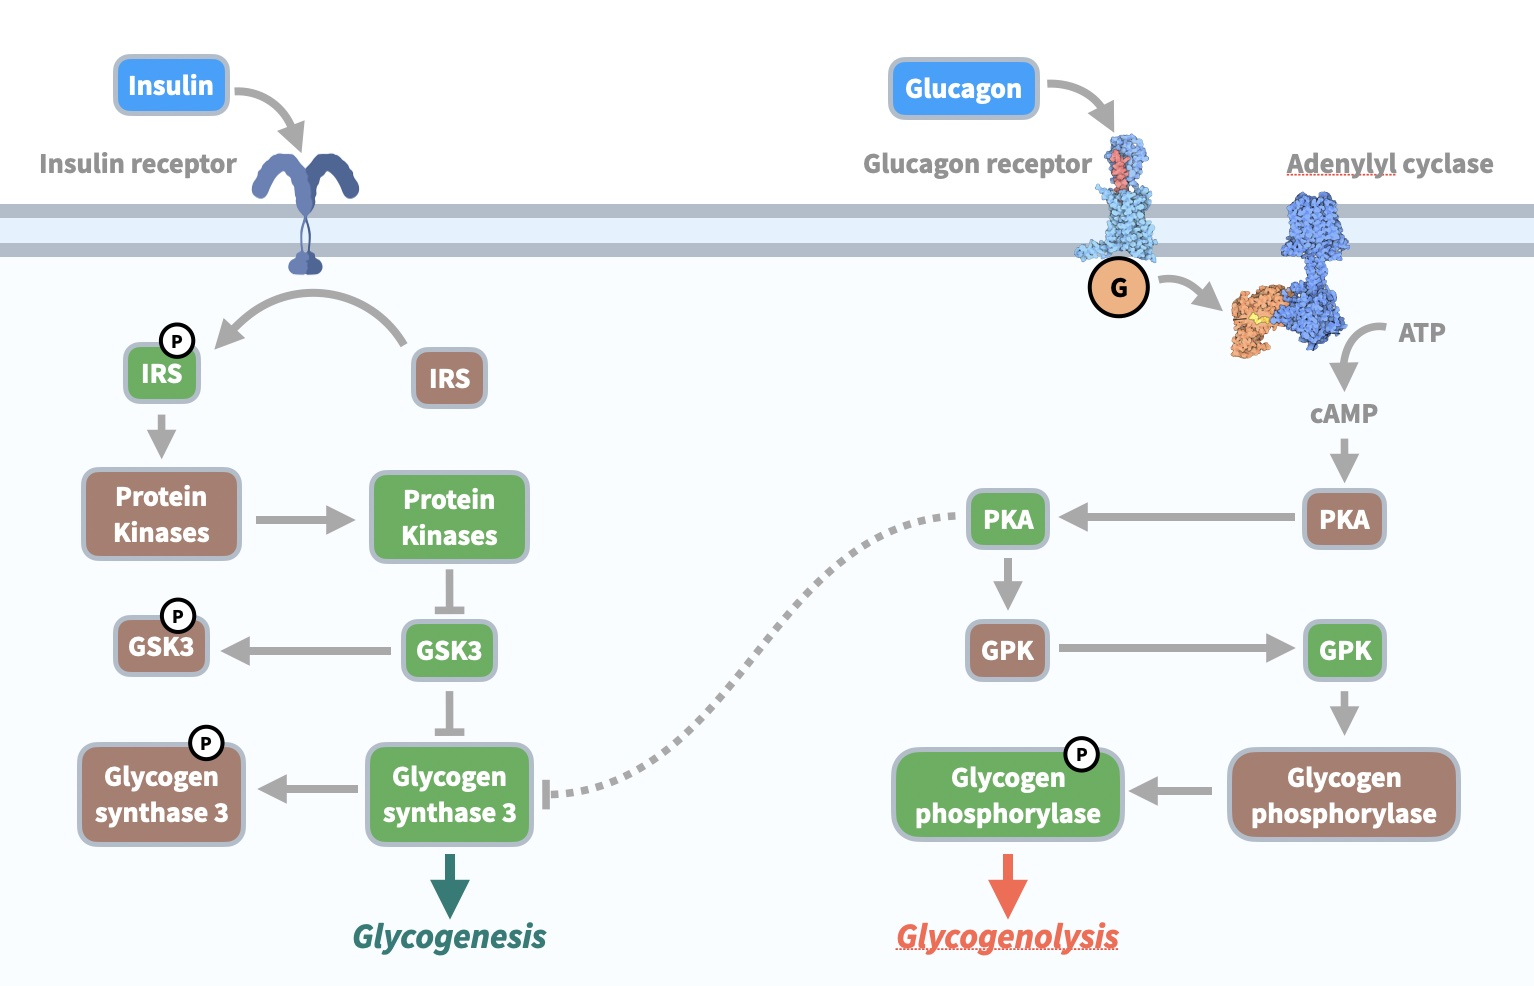
\includegraphics{img/insulin_glucagon_pathways} 

}

\caption[Insulin and Glucagon regulation of Glycogen]{Insulin and Glucagon regulation of Glycogen. This diagram illustrates one pathway by which regulation can occur.}\label{fig:unnamed-chunk-5}
\end{figure}

Here is a first example showing how glycogen storage can be reciprocally regulated by insulin and glucagon.

\subsection{Resources}\label{resources}

\begin{itemize}
\tightlist
\item
  B. Alberts et al.~\textbf{\href{https://wwnorton.com/books/9780393884821/about-the-book/product-details}{Molecular Biology of the Cell.}} (Norton, 2022, \url{ISBN:978-0-393-42708-0})
\item
  L. Szablewski \textbf{\href{https://doi.org/10.5772/67222}{Glucose Homeostasis.}} (IntechOpen, 2017, \url{DOI:10.5772/67222})
\end{itemize}



\end{document}
